\documentclass[12pt]{article}
\usepackage[a4paper,margin=1in]{geometry}
\usepackage{amsmath,amssymb}
\usepackage{graphicx}
\usepackage{siunitx}
\sisetup{per-mode=symbol}
\usepackage{gvv}

\title{Matrix 4.8.11}
\author{ai25btech11015 -- M Sai Rithik}
\date{}

\begin{document}
\maketitle

\section*{Question}
Find the vector equation of the plane determined by the points
\[
A(3,-1,2),\quad B(5,2,4),\quad C(-1,-1,6),
\]
and hence find the distance of this plane from the origin.  

\section*{Solution}

\subsection*{Step 1: Position vectors and edge vectors}
\begin{equation}
\Vec{A} = \myvec{3 \\ -1 \\ 2},\qquad
\Vec{B} = \myvec{5 \\ 2 \\ 4},\qquad
\Vec{C} = \myvec{-1 \\ -1 \\ 6}.
\end{equation}

\begin{equation}
\Vec{B}-\Vec{A} = \myvec{5 \\ 2 \\ 4} - \myvec{3 \\ -1 \\ 2}
= \myvec{2 \\ 3 \\ 2},
\end{equation}

\begin{equation}
\Vec{C}-\Vec{A} = \myvec{-1 \\ -1 \\ 6} - \myvec{3 \\ -1 \\ 2}
= \myvec{-4 \\ 0 \\ 4}.
\end{equation}

\subsection*{Step 2: Normal vector via cross product}
Using the determinant/submatrix definition of the cross product,
\begin{equation}
(\Vec{B}-\Vec{A}) \times (\Vec{C}-\Vec{A})
= \myvec{
  \mydet{\myvec{3\\2} & \myvec{0\\4}} \\[1ex]
  \mydet{\myvec{2\\2} & \myvec{-4\\4}} \\[1ex]
  \mydet{\myvec{2\\3} & \myvec{-4\\0}}
}.
\end{equation}

Now evaluate the $2\times2$ determinants:
\begin{equation}
(\Vec{B}-\Vec{A}) \times (\Vec{C}-\Vec{A})
= \myvec{ (3)(4) - (2)(0) \\[4pt] (2)(4) - (2)(-4) \\[4pt] (2)(0) - (3)(-4) }.
\end{equation}

\begin{equation}
(\Vec{B}-\Vec{A}) \times (\Vec{C}-\Vec{A})
= \myvec{12 \\ 16 \\ 12}.
\end{equation}

We may simplify (factor out 4):
\begin{equation}
\Vec{N}_0 \;=\; \myvec{3 \\ -4 \\ 3} \times (-1) \quad\text{or}\quad
\Vec{N} = \myvec{3 \\ -4 \\ 3},
\end{equation}
(we choose $\Vec{N}=(3,-4,3)^\top$, sign is arbitrary: any nonzero scalar multiple is a valid normal).

\subsection*{Step 3: Finding plane Equation}
Compute the RHS constant $d$ for the plane $\Vec{N}^{\!\top} x = d$ using point $A$:
\begin{equation}
d \;=\; \Vec{N}^{\!\top}\Vec{A}
= \begin{pmatrix}3 & -4 & 3\end{pmatrix}\myvec{3\\-1\\2}
= 3\cdot 3 + (-4)\cdot(-1) + 3\cdot 2.
\end{equation}

\begin{equation}
d = 9 + 4 + 6 = 19.
\end{equation}

Thus the plane equation in standard form is
\begin{equation}
\boxed{\; \Vec{N}^{\!\top} x = 19 \quad\text{with}\quad \Vec{N}=\myvec{3\\-4\\3}\; }.
\end{equation}


Scale the normal so that the right-hand side becomes $1$. Define
\begin{equation}
\widetilde{\Vec{N}} \;=\; \frac{\Vec{N}}{19} \;=\; \myvec{\dfrac{3}{19} \\[4pt] -\dfrac{4}{19} \\[4pt] \dfrac{3}{19}}.
\end{equation}

Then the plane can be written as
\begin{equation}
\boxed{\; \widetilde{\Vec{N}}^{\!\top} x = 1 \;},
\end{equation}
since $\widetilde{\Vec{N}}^{\!\top} x = (\Vec{N}^{\!\top}x)/19$ and $\Vec{N}^{\!\top}\Vec{A}=19$.

\subsection*{Step 5: Distance of the plane from the origin}
For a plane written as $\widetilde{\Vec{N}}^{\!\top}x = 1$, the perpendicular distance $D$ from the origin to the plane equals
\begin{equation}
D \;=\; \frac{|1|}{\|\widetilde{\Vec{N}}\|}.
\end{equation}

Compute $\|\Vec{N}\|$ first:
\begin{equation}
\|\Vec{N}\| \;=\; \sqrt{3^2 + (-4)^2 + 3^2} \;=\; \sqrt{9+16+9} \;=\; \sqrt{34}.
\end{equation}

Since $\widetilde{\Vec{N}} = \Vec{N}/19$, we have $\|\widetilde{\Vec{N}}\| = \|\Vec{N}\|/19$. Hence
\begin{equation}
D \;=\; \frac{1}{\|\widetilde{\Vec{N}}\|} \;=\; \frac{19}{\|\Vec{N}\|}.
\end{equation}

\begin{equation}
\boxed{D \;=\; \frac{19}{\sqrt{34}} \;=\; \frac{19\sqrt{34}}{34} \approx 3.260}.
\end{equation}

\section*{Final Answer}
\begin{equation}
\boxed{ \widetilde{\Vec{N}}^{\!\top} x = 1,\quad
\widetilde{\Vec{N}} = \myvec{\dfrac{3}{19} \\[4pt] -\dfrac{4}{19} \\[4pt] \dfrac{3}{19}}, }
\end{equation}
\begin{equation}
\boxed{ \text{Distance from origin to plane} = \dfrac{19}{\sqrt{34}} \approx 3.260. }
\end{equation}

\begin{figure}[h!]
    \centering
    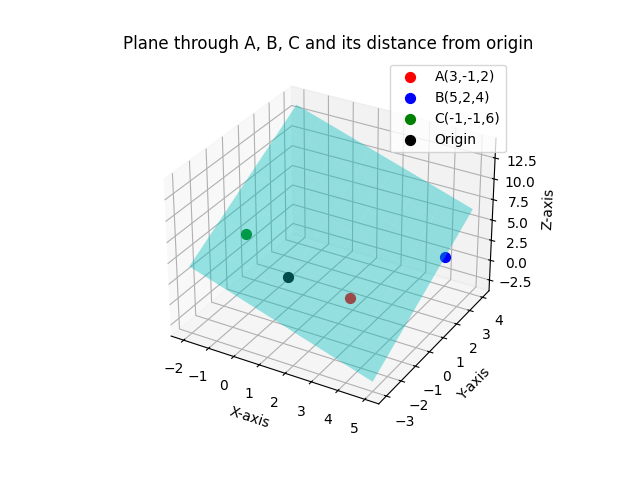
\includegraphics[width=0.65\linewidth]{figs/fig.png}
    \caption{}
\end{figure}

\end{document}
